\documentclass[10pt,aspectratio=169]{beamer}

% All the boilerplate is in raslides.sty
% Note that this also pulls in a custom vogtwidebar.sty
\usepackage{raslides}

\author{Ji\v{r}\'i Lebl}

\institute[OSU]{%
Departemento pri Matematiko de Oklahoma {\^S}tata Universitato}

\title{BA: 2.1}

\date{}

\begin{document}

\begin{frame}
\titlepage
\end{frame}

\begin{frame}
\begin{definition}
A \emph{sequence} (in $\R$) is a function $x \colon \N \to
\R$.  Instead of $x(n)$, we write $x_n$.  For the whole sequence
we write
\begin{equation*}
\{ x_n \}_{n=1}^\infty .
\end{equation*}
\pause
$\{ x_n \}_{n=1}^\infty$ is \emph{bounded} if
$\exists$ a $B \in \R$ such that
\quad
$\abs{x_n} \leq B$ \quad for all $n \in \N$.
\end{definition}

\pause

\textbf{Example:}
$\{ \nicefrac{1}{n} \}_{n=1}^\infty$ stands for
$1, \nicefrac{1}{2}, \nicefrac{1}{3}, \nicefrac{1}{4}, \nicefrac{1}{5}, \ldots$.

\pause
$\{ \nicefrac{1}{n} \}_{n=1}^\infty$
is a bounded sequence ($B=1$ suffices).

\medskip
\pause

$\{ n \}_{n=1}^\infty$ stands for
$1,2,3,4,\ldots$, and this sequence is not bounded (why?).

\medskip
\pause

If $c \in \R$ is a constant, then $\{ c \}_{n=1}^\infty$
is the \emph{constant sequence}
$c,c,c,c,\ldots$

\medskip
\pause

Be careful to distinguish sets and sequences:

$\{ {(-1)}^n \}_{n=1}^\infty$ is the sequence
$-1,1,-1,1,-1,1,\ldots$, whereas the set of its values, the
\emph{range of the sequence},
is the set $\{ -1, 1 \}$.

\end{frame}

\begin{frame}
\begin{definition}
A sequence $\{ x_n \}_{n=1}^\infty$ is said to \emph{converge} to
$x \in \R$ if for every $\epsilon > 0$, there exists an $M \in \N$ such
that $\abs{x_n - x} < \epsilon$ for all $n \geq M$.
\pause

Call $x$ a \emph{limit} of $\{ x_n \}_{n=1}^\infty$ and (if unique) write
\begin{equation*}
\lim_{n\to \infty} x_n \coloneqq x .
\end{equation*}
\pause
A sequence
that converges is \emph{convergent}.
Otherwise, it \emph{diverges}, or is \emph{divergent}.
\end{definition}

\pause

We will prove momentarily that the limit,
if it exists, is always unique.

\pause
\medskip

Limits do not always exist.
\pause
Writing down ``$\lim\limits_{n\to\infty} x_n = x$'' means two things:

1) The limit exists.

2) It equals $x$.

\pause
\medskip

\textbf{Remark:}
The limit $x$ may or may not be one of the numbers in the sequence.

\pause
\medskip

Note the dependence: $M$ may depend on $\epsilon$.  We only need to pick $M$
once we know $\epsilon$.
\end{frame}

\begin{frame}
\centering
\scalebox{0.9}{
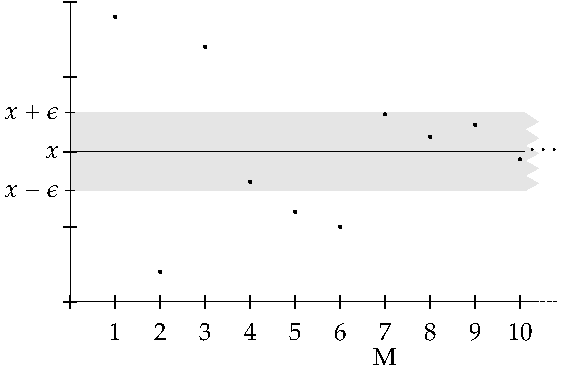
\includegraphics{../figures/sequence-convergence}
}

\medskip

\scalebox{0.9}{
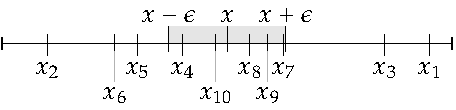
\includegraphics{../figures/sequence-convergence-2}
}
\end{frame}

\begin{frame}
\textbf{Example:}
$\{ 1 \}_{n=1}^\infty$ converges to 1.  \pause 

\textbf{Proof:} Given $\epsilon > 0$, let $M=1$.

\pause
Then for $n \geq M=1$, \quad
$\abs{x_n-x} = \abs{1-1} = 0 < \epsilon$. \qed

\medskip
\pause

\textbf{Example:}
$\{ \nicefrac{1}{n} \}_{n=1}^\infty$ converges to 0.

\pause
\textbf{Proof:} Given $\epsilon > 0$, find $M$ such that
$0 < \nicefrac{1}{M} < \epsilon$ (Archimedean property).

\pause
Then for all $n \geq M$,
\quad
$\abs{x_n - x}
\pause
= \abs{\frac{1}{n} - 0}
\pause
= \abs{\frac{1}{n}}
\pause
= \frac{1}{n}
\pause
\leq \frac{1}{M}
\pause < \epsilon$. \qed

\medskip
\pause

\textbf{Example:}
$\{ {(-1)}^n \}_{n=1}^\infty$ is divergent.

\pause
\textbf{Proof:} Suppose $x$ is a limit.  Find $M$ for $\epsilon = \frac{1}{2}$.

\pause
For even $n \geq M$,
\quad
$\nicefrac{1}{2} > \abs{x_n - x} \pause  = \abs{1 - x}$
\pause
\quad  and \quad 
$\nicefrac{1}{2} > \abs{x_{n+1} - x} \pause  = \abs{-1 - x}$.

\pause
But
\quad
$2 = \abs{1 - x - (-1 -x)} \pause \leq \abs{1 - x} + \abs{-1 -x} \pause <
\nicefrac{1}{2} + \nicefrac{1}{2} = 1$.

\pause
A contradiction. \qed
\end{frame}

\begin{frame}

\begin{proposition}
A convergent sequence has a unique limit.
\end{proposition}

\pause

\textbf{Proof:}
Suppose $\{ x_n \}_{n=1}^\infty$ has limits $x$ and $y$.

\pause
Take an arbitrary $\epsilon > 0$.

\pause
Find an $M_1$ such that for all $n \geq M_1$,
\quad
$\abs{x_n-x} < \nicefrac{\epsilon}{2}$.


\pause
Find an $M_2$ such that for all $n \geq M_2$,
\quad
$\abs{x_n-y} < \nicefrac{\epsilon}{2}$.

\pause
Consider $n$ such that $n \geq M_1$ \textbf{and} $n \geq M_2$.

\pause
$
\abs{y-x}
\pause =
\abs{x_n-x - (x_n -y)}
\pause \leq
\abs{x_n-x} + \abs{x_n -y}
\pause <
\frac{\epsilon}{2} + \frac{\epsilon}{2} = \epsilon .
$

\pause
$\abs{y-x} < \epsilon$ $\forall$  $\epsilon > 0$ \wthus $\abs{y-x} = 0$
\pause
\wthus $y=x$.

\pause
Hence the limit (if it exists) is unique.
\qed

\medskip
\pause

\textbf{Remark:} Note the technique.  A quantity to be shown as zero is
written as a sum of two things that are small.
\end{frame}

\begin{frame}

\begin{proposition}
A convergent sequence $\{ x_n \}_{n=1}^\infty$ is bounded.
\end{proposition}

\pause

\textbf{Proof:}
Suppose $\{ x_n \}_{n=1}^\infty$ converges to $x$.

\pause
\thus \quad $\exists$ an $M \in \N$ such that for all $n \geq M$,\quad
$\abs{x_n - x} < 1$.

\medskip
\pause

For $n \geq M$, \quad
$\abs{x_n} = \abs{x_n - x + x} \pause
\leq \abs{x_n - x} + \abs{x} \pause
< 1 + \abs{x}$.

\medskip
\pause

$\bigl\{ \abs{x_1}, \abs{x_2}, \ldots, \abs{x_{M-1}}, 1+\abs{x} \bigr\}$
is a finite set,

so let
\quad $B \coloneqq \max \bigl\{ \abs{x_1}, \abs{x_2}, \ldots, \abs{x_{M-1}}, 1+\abs{x} \bigr\}$.

\medskip
\pause

Then for all $n \in \N$, \quad $\abs{x_n} \leq B$.
\qed

\medskip
\pause

Converse does not hold: $\{ {(-1)}^n \}_{n=1}^\infty$ is bounded but not convergent.

\end{frame}

\begin{frame}


\textbf{Example:}
We claim $\left\{ \frac{n^2+1}{n^2+n} \right\}_{n=1}^\infty$ converges and
\quad $\displaystyle \lim_{n\to\infty} \frac{n^2+1}{n^2+n} = 1$.

\medskip
\pause

\textbf{Proof:}
Given $\epsilon > 0$, find $M \in \N$ such that $\frac{1}{M} < \epsilon$.

\medskip
\pause

For all $n \geq M$,

\medskip

\qquad
$\displaystyle
\abs{\frac{n^2+1}{n^2+n} - 1}  \pause = \abs{\frac{n^2+1 - (n^2+n)}{n^2+n}}
\pause
=
\abs{\frac{1 - n}{n^2+n}}
\pause
=
\frac{n-1}{n^2+n}
%$
%
%\medskip
\pause
%
%\hfill
%$\displaystyle
\leq 
\frac{n}{n^2+n} 
\pause
 =
\frac{1}{n+1}
\pause
\leq \frac{1}{n}
\pause
\leq \frac{1}{M}
\pause < \epsilon .
$\qquad

\medskip
\pause

\thus \quad
$\lim\limits_{n\to\infty} \dfrac{n^2+1}{n^2+n} = 1$. \qed

\medskip
\pause

\textbf{Remark:} Sometimes you throw something away
to make things simpler.

\pause
Just don't throw away too much.

\end{frame}

\begin{frame}
\begin{definition}
A $\{ x_n \}_{n=1}^\infty$ is \emph{monotone increasing} if $x_n \leq x_{n+1}$ for all $n \in \N$.  

\pause
A $\{ x_n \}_{n=1}^\infty$ is \emph{monotone decreasing} if $x_n \geq x_{n+1}$ for all $n \in \N$.  

\pause
If it is one of the two, but doesn't matter which, just say it is \emph{monotone}.
\end{definition}

\pause

Monotone sequences are easier to handle.

\medskip
\pause

\textbf{Examples:}

\pause
$\{ n \}_{n=1}^\infty$ is monotone increasing,

\pause
$\{ \nicefrac{1}{n} \}_{n=1}^\infty$ is monotone decreasing,

\pause
$\{ 1 \}_{n=1}^\infty$ (constant) is both monotone increasing and monotone decreasing,

\pause
$\{ {(-1)}^n \}_{n=1}^\infty$ is not monotone.

\end{frame}

\begin{frame}
\textbf{Example:} Monotone increasing sequence:

\begin{center}
\scalebox{0.9}{
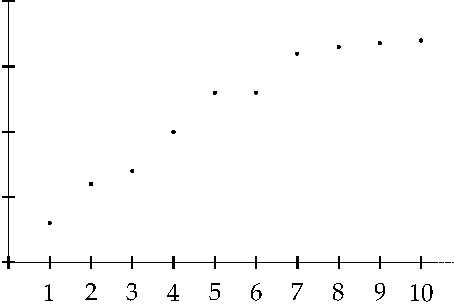
\includegraphics{../figures/sequence-increasing}
}
\end{center}

\end{frame}

\begin{frame}

\begin{proposition}
A monotone sequence $\{ x_n \}_{n=1}^\infty$ is bounded if and only if it is convergent.

\pause
If $\{ x_n \}_{n=1}^\infty$ is monotone increasing and bounded, then \quad
$\displaystyle
\lim_{n\to \infty} x_n = \sup \{ x_n : n \in \N \}$.

\pause
If $\{ x_n \}_{n=1}^\infty$ is monotone decreasing and bounded, then \quad
$\displaystyle
\lim_{n\to \infty} x_n = \inf \{ x_n : n \in \N \}$.
\end{proposition}

\pause

\textbf{Proof:}
Consider a monotone increasing $\{x_n\}_{n=1}^\infty$.  First suppose it is bounded.

\pause
The set $\{ x_n : n \in  \N \}$ is bounded, so let
\quad $x \coloneqq \sup \{ x_n : n \in \N \}$.

\pause
Let $\epsilon > 0$ be arbitrary.

\pause
$\exists$ $M \in \N$ such that $x_{M} > x-\epsilon$ \quad (as $x$ is the supremum).

\pause
As $\{ x_n \}_{n=1}^\infty$ is monotone increasing (by induction),
\quad $x_n \geq x_M$ for all $n \geq M$.

\pause
\thus \quad for all $n \geq M$,
\quad $\abs{x_n-x} = x-x_n \leq x-x_{M} < \epsilon$.

\pause
\thus \quad $\{x_n \}_{n=1}^\infty$ converges to $x$.

\medskip
\pause

On the other hand, we already proved a convergent sequence is bounded.

\medskip
\pause

Monotone decreasing left as exercise.
\qed

\end{frame}

\begin{frame}

\textbf{Example:}
Consider $\bigl\{ \frac{1}{\sqrt{n}} \bigr\}_{n=1}^\infty$.

\medskip
\pause

$\frac{1}{\sqrt{n}} > 0$ for all $n \in \N$, so bounded below.

\pause
$\forall$ $n \in \N$, ~
$\sqrt{n+1} \geq \sqrt{n}$ (why?)
\pause
~\thus~
$\dfrac{1}{\sqrt{n+1}} \leq \dfrac{1}{\sqrt{n}}$
\pause
~\thus~
monotone decreasing

\medskip
\pause
\thus \quad convergent (by proposition) and

\medskip
\pause

$\displaystyle
\lim_{n\to \infty} \frac{1}{\sqrt{n}}
=
\inf \left\{ \frac{1}{\sqrt{n}} : n \in \N \right\}$

\medskip
\pause

$0$ is a lower bound \wthus the infimum is $\geq 0$.

\medskip
\pause

Suppose $b \geq 0$ such that 
$b \leq \frac{1}{\sqrt{n}}$ for all $n \in \N$.

\pause
\thus \quad
$b^2 \leq \frac{1}{n}$ for all $n \in \N$.

\pause
\medskip

We proved before that this means $b^2 \leq 0$ (Archimedean property).

\pause
\medskip

As $b^2 \geq 0$ as well \wthus $b^2 = 0$ \pause \wthus $b=0$.

\pause
\medskip

So $b=0$ is the greatest lower bound \pause\wthus
$\lim\limits_{n\to\infty} \frac{1}{\sqrt{n}} = 0$.
\end{frame}

\begin{frame}
\textbf{Example:}
$\{ 1 + \nicefrac{1}{2} + \cdots + \nicefrac{1}{n} \}_{n=1}^\infty$ is monotone and seems to grow very
slowly.

\medskip
\pause

$1 + \nicefrac{1}{2} + \nicefrac{1}{3} + \cdots + \nicefrac{1}{10} \approx
2.92897$

\medskip
\pause

$1 + \nicefrac{1}{2} + \nicefrac{1}{3} + \cdots + \nicefrac{1}{100} \approx
5.18738$

\medskip
\pause

$1 + \nicefrac{1}{2} + \nicefrac{1}{3} + \cdots + \nicefrac{1}{1000} \approx
7.48547$

\medskip
\pause

$1 + \nicefrac{1}{2} + \nicefrac{1}{3} + \cdots + \nicefrac{1}{1001} \approx
7.48647$

\medskip
\pause

$1 + \nicefrac{1}{2} + \nicefrac{1}{3} + \cdots + \nicefrac{1}{1002} \approx
7.48747$

\medskip
\pause

So once we're up to $n \approx 1000$, we're only changing in the third
decimal place.

\medskip
\pause

\textbf{However,}
we'll see later that it does not converge.  It is unbounded!

\end{frame}

\begin{frame}
Monotone sequences appear naturally in computing superma/infima:

\pause

\begin{proposition}
Let $S \subset \R$ be a nonempty bounded set.
\pause
Then $\exists$ monotone sequences
$\{ x_n \}_{n=1}^\infty$ and $\{ y_n \}_{n=1}^\infty$ such that $x_n, y_n \in S$ and
\begin{equation*}
\sup\,S = \lim_{n\to \infty} x_n \qquad \text{and} \qquad \inf\,S =
\lim_{n\to\infty} y_n .
\end{equation*}
\end{proposition}

\pause

Proof is an exercise.
\end{frame}

\begin{frame}

\begin{definition}
For a sequence $\{ x_n \}_{n=1}^\infty$,
the \emph{$K$-tail} (where $K \in \N$),
or just the
\emph{tail}, of
$\{ x_n \}_{n=1}^\infty$ is the sequence starting at $K+1$, usually written as
\begin{equation*}
\{ x_{n+K} \}_{n=1}^\infty
\qquad \text{or} \qquad \{ x_n \}_{n=K+1}^\infty .
\end{equation*}
\end{definition}

\pause

\textbf{Example:}
The $4$-tail of $\{ \nicefrac{1}{n} \}_{n=1}^\infty$ is

$\nicefrac{1}{5}, \nicefrac{1}{6}, \nicefrac{1}{7}, \nicefrac{1}{8},
\ldots$.

\medskip
\pause

The $0$-tail of a sequence is the sequence itself.

\medskip
\pause

The reason for studying tails is that convergence only depends on the tail.

\end{frame}

\begin{frame}[fragile]

\begin{proposition}
Let $\{ x_n \}_{n=1}^\infty$ be a sequence.  Then the following
statements are equivalent:
\begin{enumerate}[(i)]
\item \label{prop:ktail:i}
The sequence $\{ x_n \}_{n=1}^\infty$ converges.
\item \label{prop:ktail:ii}
The $K$-tail $\{ x_{n+K} \}_{n=1}^\infty$ converges for all $K \in \N$.
\item \label{prop:ktail:iii}
The $K$-tail $\{ x_{n+K} \}_{n=1}^\infty$ converges for some $K \in \N$.
\end{enumerate}
Furthermore, if any (and hence all) of the limits exist, then for all $K \in \N$
\begin{equation*}
\lim_{n\to \infty} x_n = \lim_{n \to \infty} x_{n+K} .
\end{equation*}
\end{proposition}

\pause

\textbf{Proof:}
\eqref{prop:ktail:ii} \thus \eqref{prop:ktail:iii} is immediate.

\medskip
\pause

The logic of the proof is
\begin{equation*}
\begin{tikzcd}[row sep=0pt]
& \text{\eqref{prop:ktail:ii}} \ar[dr, Rightarrow] & \\
\text{\eqref{prop:ktail:i}} \ar[ur, Rightarrow, "\text{to prove}"] & &
\text{\eqref{prop:ktail:iii}} \ar[ll, Rightarrow, "\text{to prove}"] 
\end{tikzcd}
\end{equation*}

\medskip
\pause

We will also show that the limits are equal.

\end{frame}

\begin{frame}
Start with ``\eqref{prop:ktail:i} \thus \eqref{prop:ktail:ii}.''

\pause
Suppose $\{x_n \}_{n=1}^\infty$ converges to $x \in \R$, and let $K \in \N$ be arbitrary.

\pause
Given an $\epsilon > 0$, $\exists$ $M \in \N$ such that
$\sabs{x-x_n} < \epsilon$ for all $n \geq M$.

\pause
Note that $n \geq M$ implies $n+K \geq M$.

\pause
\thus \quad for all $n \geq M$, \quad
$\sabs{x-x_{n+K}} < \epsilon$.

\pause
\thus \quad The $K$-tail converges to $x$.

\medskip
\pause

Let us prove ``\eqref{prop:ktail:iii} \thus \eqref{prop:ktail:i}.''

\pause
Let $K \in \N$ be given and suppose $\{ x_{n+K} \}_{n=1}^\infty$ converges to $x \in \R$.

\pause
Given an $\epsilon > 0$, $\exists$ $M' \in \N$ such that
$\sabs{x-x_{n+K}} < \epsilon$ for all $n \geq M'$.

\pause
Let $M \coloneqq M'+K$.

\pause
$n \geq M$ \wthus $n-K \geq M'$.

\pause
\thus \quad for all $n \geq M$, \quad
$\sabs{x-x_n} = \sabs{x-x_{(n-K)+K}} < \epsilon$.

\pause
\thus \quad $\{ x_n \}_{n=1}^\infty$ converges to $x$.
\qed

\end{frame}

\begin{frame}
So the limit does not care how the sequence begins.

\medskip
\pause

\textbf{Example:}
\medskip

$\bigl\{\frac{n}{n^2+16} \bigr\}_{n=1}^\infty =
\nicefrac{1}{17},
\nicefrac{1}{10},
\nicefrac{3}{25},
\nicefrac{1}{8},
\nicefrac{5}{41},
\nicefrac{3}{26},
\nicefrac{7}{65},
\nicefrac{1}{10},
\nicefrac{9}{97},
\nicefrac{5}{58},\ldots$

\pause
\medskip

$
\nicefrac{1}{17} <
\nicefrac{1}{10} <
\nicefrac{3}{25} <
\nicefrac{1}{8} >
\nicefrac{5}{41} >
\nicefrac{3}{26} >
\nicefrac{7}{65} >
\nicefrac{1}{10} >
\nicefrac{9}{97} >
\nicefrac{5}{58} > \ldots$

\medskip
\pause

$\bigl\{\frac{n}{n^2+16} \bigr\}_{n=1}^\infty$ is monotone decreasing (exercise) if we start with $n=4$.

\medskip
\pause

So the 3-tail is monotone.

\medskip
\pause

It is also bounded below (all terms are positive).

\medskip
\pause

So it is convergent.
\end{frame}

\begin{frame}
\begin{definition}
Let $\{ x_n \}_{n=1}^\infty$ be a sequence.

\pause
Let $\{ n_i \}_{i=1}^\infty$ be a strictly increasing sequence of natural
numbers, that is, $n_i < n_{i+1}$ for all $i$ (in other words $n_1 < n_2 < n_3 < \cdots$).  

\pause
The sequence
\quad $\{ x_{n_i} \}_{i=1}^\infty$ \quad
is a \emph{subsequence} of $\{ x_n \}_{n=1}^\infty$.
\end{definition}

\pause

The subsequence is the sequence $x_{n_1},x_{n_2},x_{n_3},\ldots$.

\medskip
\pause

\textbf{Example:} $\{ \nicefrac{1}{n} \}_{n=1}^\infty$

\pause
$\{ \nicefrac{1}{3i} \}_{i=1}^\infty =
\nicefrac{1}{3},\nicefrac{1}{6},\nicefrac{1}{9},\nicefrac{1}{12}\ldots$ is a subsequence.

\pause
Use $n_i = 3i$ in the definition.

\medskip
\pause

$1,0,\nicefrac{1}{3},0, \nicefrac{1}{5},\ldots$ is \textbf{not} a
subsequence of $\{ \nicefrac{1}{n} \}_{n=1}^\infty$.

\medskip
\pause

$1,\nicefrac{1}{3},\nicefrac{1}{2},\nicefrac{1}{5},\ldots$
is \textbf{not} a subsequence of $\{ \nicefrac{1}{n} \}_{n=1}^\infty$.

\end{frame}

\begin{frame}

A tail of a sequence is a subsequence.

\medskip
\pause

For general subsequences we have the following proposition on convergence.

\pause

\begin{proposition}
If $\{ x_n \}_{n=1}^\infty$ is a convergent sequence,
then every subsequence $\{ x_{n_i} \}_{i=1}^\infty$ is also convergent, and
\[
\lim_{n\to \infty} x_n = 
\lim_{i\to \infty} x_{n_i} .
\]
\end{proposition}

\pause

\textbf{Proof:}
Let $x \coloneqq \lim\limits_{n\to \infty} x_n$.

\medskip
\pause
Given $\epsilon > 0$, $\exists$ $M \in \N$ such that for all $n \geq M$,
$\abs{x_n - x} < \epsilon$.

\medskip
\pause
By induction (try it), $n_i \geq i$.

\medskip
\pause
So \quad $i \geq M$ \wthus $n_i \geq M$.

\medskip
\pause
\thus \quad for all $i \geq M$, \quad
$\abs{x_{n_i} - x} < \epsilon$.
\qed

\end{frame}

\begin{frame}

\textbf{Example:}
Existence of a convergent subsequence does not imply
convergence of the sequence itself.

\medskip
\pause
Consider $0,1,0,1,0,1,\ldots$ \quad
($x_n = 0$ if $n$ is odd, and $x_n = 1$ if $n$ is even)

\medskip
\pause

$\{ x_n \}_{n=1}^\infty$ is divergent.

\medskip
\pause

$\{ x_{2i} \}_{i=1}^\infty$ converges to 1.

\medskip
\pause

$\{ x_{2i+1} \}_{i=1}^\infty$ converges to 0.
\end{frame}

\end{document}
